\section{Introduction}
\label{sec:introduction}

The Baum--Connes assembly map relates the topology of a discrete group to
the operator algebra generated by its regular representation.  For a
torsion-free discrete group $\Ginj$, its coefficient-free form is
\[
  \mu_{\Ginj}^r\colon K_*(B\Ginj)\longrightarrow K_*(C_r^*(\Ginj)).
\]
Here $B\Ginj$ is a classifying space, $K_*(B\Ginj)$ is complex topological
$K$-homology with compact support, namely the directed limit over finite
subcomplexes, and $C_r^*(\Ginj)$ is the reduced group $C^*$-algebra.  The
Baum--Connes conjecture asserts that this map is an isomorphism
\cite{BCH94}.  In this formulation the coefficient algebra is
$\mathbb C$ with its trivial action; the more general conjecture with
coefficients allows a $\Ginj$-algebra $A$ and has target $K_*(A\rtimes_r \Ginj)$.

\begin{theorem}\label{thm:main}
There exist a finitely generated torsion-free discrete group \(\Ginj\), an injective homomorphism \(i:\Z^2\to \Ginj\), and a class \(c\in H^2(B\Ginj;\Z)\) such that
\[
\ip{(Bi)^*c}{[T^2]}=1,\qquad
i_*(\beta)=0\quad\text{in }K_0(\Cr \Ginj),
\]
where \(\beta\) is a rank-zero Bott generator of \(K_0(\Cr\Z^2)\).
In particular, \(h=(Bi)_*[D_{T^2}]\) has infinite order in \(K_0(B\Ginj)\), while its reduced analytic assembly image is zero. Here \([D_{T^2}]\) is the spin Dirac \(K\)-homology class of the oriented torus.
\end{theorem}

The theorem gives an integral reduced assembly kernel class of infinite
order, and hence disproves rational injectivity of coefficient-free reduced
assembly. Its two assertions have different roles. The cohomology class
extends the orientation class of the embedded torus and detects its Dirac
class by an index pairing. The vanishing of the corresponding rank-zero
Bott class is proved by a separate operator-algebra construction.
The group is finitely generated; finite presentation is not part of the
conclusion.

\subsection{The distinction from earlier counterexamples}

Baum and Connes introduced this index-theoretic comparison in a preprint
circulated in 1982 and published in 2000
\cite[Section~1 and editors' note]{BC00}. The formulation using the
classifying space for proper actions was developed with Higson
\cite[Conjecture~3.15]{BCH94}. In the torsion-free case that space gives
the assembly map displayed above.

The conjecture is known for substantial classes of groups. Higson and
Kasparov prove it with separable coefficients for groups acting properly by affine
isometries on Hilbert space, including countable amenable groups
\cite[Theorem~9.1 and Corollary~9.2]{HK01}. The coefficient-free hyperbolic
case was established by Mineyev--Yu using Lafforgue's Banach-$KK$ methods
\cite[Theorem~20]{MY02}; Lafforgue subsequently proved the version with
coefficients \cite[Theorem~0.4]{Laf12}. Guentner, Higson, and Weinberger
prove split injectivity with coefficients for countable linear groups
\cite[Theorem~3]{GHW05}. These results describe major settings where the kernel
constructed here cannot occur.


Higson, Lafforgue, and Skandalis constructed counterexamples in several
assembly settings \cite{HLS02}.  For discrete groups, their examples
concern failure of surjectivity with nontrivial commutative coefficients;
their paper explicitly distinguishes this from the conjecture for groups
alone.  Its groupoid examples also have failures of injectivity, but the
groupoid and coefficient-free group assertions have different domains
and targets.  Theorem~\ref{thm:main} concerns injectivity with coefficient
algebra $\mathbb C$.

Gromov's graph-labeled small-cancellation strategy connects expander
geometry to group constructions \cite[\S4.8]{Gro03}.
Graphical small-cancellation methods subsequently gave further group
constructions with coefficient obstructions.  For example,
Osajda's graphical constructions, together with the coefficient result of
Willett and Yu, give a suitable coefficient algebra for which reduced
assembly is injective and not surjective
\cite[Corollary~3.4]{Osa20}\cite[Corollary~1.7]{WY12}.
This provides relevant geometric precedent without supplying the
coefficient-free kernel required here.

The exact crossed-product reformulation of Baum, Guentner, and Willett
was designed to address the failures involving coefficients
\cite{BGW16}.  It replaces the reduced crossed product by the minimal
exact Morita-compatible crossed product.  That reformulation, the reduced
coefficient-free conjecture, and the maximal assembly map must be kept
distinct when interpreting the present construction.

\subsection{Maximal assembly and the Novikov conjecture}

Write $\mu_{\Ginj}^{\max}$ for assembly with target $K_*(C^*_{\max}(\Ginj))$,
and let $\lambda_{\Ginj}$ be the regular quotient from $C^*_{\max}(\Ginj)$ to
$C_r^*(\Ginj)$.  By the completion comparison
\cite[Remark~2.6]{Land15},
\[
  \mu_{\Ginj}^r=(\lambda_{\Ginj})_*\mu_{\Ginj}^{\max}.
\]
Hanke and Schick prove maximal rational nonvanishing for every discrete
group whenever a $K$-homology class is detected by the subring of rational
cohomology generated in degrees at most two
\cite[Theorem~1.2]{HS08}.  Consequently the class $h$ in
Theorem~\ref{thm:main} satisfies
\[
  \mu_{\Ginj}^{\max}(h)\otimes1\ne0,
  \qquad
  (\lambda_{\Ginj})_*\bigl(\mu_{\Ginj}^{\max}(h)\bigr)=0.
\]
The name \emph{strong Novikov conjecture} is used for both maximal and
reduced rational injectivity in the literature
\cite[Section~7]{BCH94}\cite[Section~8.3, footnote~6]{BGW16}.
Theorem~\ref{thm:main} disproves the reduced formulation, while maximal
assembly detects the same class $h$. The classical Novikov conjecture
concerns oriented homotopy invariance of higher signatures. Our result
disproves neither maximal rational injectivity nor this classical
assertion; in particular, higher signatures associated to
low-degree cohomology already have the homotopy invariance established in
\cite[Corollary~1.3]{HS08}.

Antonini, Buss, Engel, and Siebenand extend the low-degree nonvanishing
result to suitable exotic group $C^*$-algebras
\cite[Theorem~B]{ABES21}.  Their corrected statement assumes a
\emph{finitely presented} group and applies, in particular, to the group
algebra of the minimal exact Morita-compatible crossed-product functor.
For exact groups this algebra agrees with the reduced group algebra.
The asserted agreement for all groups was affected by the gap recorded
in the erratum of Buss, Echterhoff, and Willett \cite{BEW21err}.
Accordingly we use the corrected version of \cite{ABES21},
arXiv:1905.07730v3, rather than its original reduced-algebra claim.
Theorem~\ref{thm:main} asserts finite generation; it supplies neither
finite presentation nor exactness.

A further distinction concerns projections.  For a countable
torsion-free group, a nontrivial projection in the scalar algebra
$C_r^*(\Ginj)$ would obstruct surjectivity of coefficient-free assembly
\cite[Corollary~1.6]{KP22}.  Such a projection alone does not identify
an assembly kernel class.  Here matrix-valued Bott representatives are
used to prove a specific vanishing while the integral detector proves
that the corresponding geometric class survives.

\subsection{The construction}

In the operator model, localized rank-zero Bott representatives occupy
coordinates indexed by heights $i\geq0$. The analytic aim is to cancel
the class at height zero by moving bounded families of these
representatives. Rotations and
rescalings on the disjoint adjacent pairs $(0,1),(2,3),\ldots$ move
the even family to the odd family. The pairs $(1,2),(3,4),\ldots$
then move the odd family to the positive-even family. These two
homotopies identify the even family with the family obtained by removing
its height-zero term. Finite additivity therefore forces that term to
vanish. The families must be actual bounded operators, their homotopies
must belong to a reduced-algebra norm quotient, and the resulting
equality must yield a finite witness in one group algebra. These
requirements determine the construction below.

The proof connects three ingredients. Its graph-labeling stage is related
to the finite-alphabet separation method of Osajda \cite[\S2]{Osa20}; the
layered graph, the sequential expansion constraints, and the simultaneous
spectral requirements below are additional features. The voltage-cover
language follows Gross and Gross--Tucker \cite{Gross74,GT77}. Neither
reference supplies the analytic realization needed here.

First, a layered graph is labeled by interleaved finite streams.
Two incident labels recover successive blocks of a vertex state.
The recovery procedure gives uniqueness for sufficiently long immersed
words, while the random tables can be selected with a uniform expansion
gap. Products of these incidences and their adjoints will later isolate
the normalized constant coordinates on which the Bott families act.
Pruning removes short coherent returns and configurations that
would obstruct the required overlap bounds.  The central issue is to
retain enough independent constraints after conditioning on expansion.
Proposition~\ref{prop:tower-labels},
Proposition~\ref{prop:sequential-law}, and
Proposition~\ref{prop:pruning} give the labeling, selection law, and
counting estimates with compatible parameters.

Second, the graph is given voltages in the integral Heisenberg group
\[
  \mathsf H=\langle x,y,z\mid [x,y]=z,\ [x,z]=[y,z]=1\rangle.
\]
A voltage assigns a group element $h_e$ to an oriented base edge
$v\to w$; its lift sends $(v,f)$ to $(w,fh_e)$, and the reverse edge
uses $h_e^{-1}$.
Short circuits surviving pruning are not laws in $\mathsf H$.
The voltage choice simultaneously separates these circuits and
approximates the required spectral averages.  Continuous matrix-valued
symbols spread the Bott class across spectral bands, and finite
sampling is controlled in the full regular operator norm.
Proposition~\ref{prop:sampled-symbols} supplies this analytic selection.
The Heisenberg group provides a torsion-free source for the voltage
cover and also contains the commuting pair $(z,x)$ used for the final
torus.

Third, the geometric realization keeps the Heisenberg subgroup embedded
and makes its degree-two detector extend to the ambient group.  A
\emph{sheet} is a translate of the embedded cover in the Cayley graph.
Integral cycle decompositions in a complex built from these sheets
control both torsion and restriction in cohomology; see
Proposition~\ref{prop:graphical-realization} and
Proposition~\ref{prop:torsion-detector}. Disjoint domains in the sheets
allow the spectral operators to act on the group's regular Hilbert
space. The number of excluded coordinates in each sheet is bounded,
and the spectral support projections have traces small enough relative
to these bounds that the loss on the supported operators is small in
norm. The remaining Cayley edges
form a forest, whose contribution is controlled by the ratio of the
square root of the label count to the incidence normalizer. This is why
the finite alphabet must retain a sharp margin throughout the graph
construction. These estimates realize the bounded Bott families and
their homotopies in the reduced-algebra norm quotient.
Proposition~\ref{prop:reduced-bott-vanishing} then obtains integral
Bott vanishing in an actual reduced group algebra. The finite-witness
argument retains this equality in the group generated
by the finitely many group elements in polynomial approximations to that
witness, together with the Heisenberg generators. This finitely
generated subgroup is the group in Theorem~\ref{thm:main}.

Figure~\ref{fig:proof-dependencies} records the main dependencies.
\begin{figure}[tbp]
  \centering
  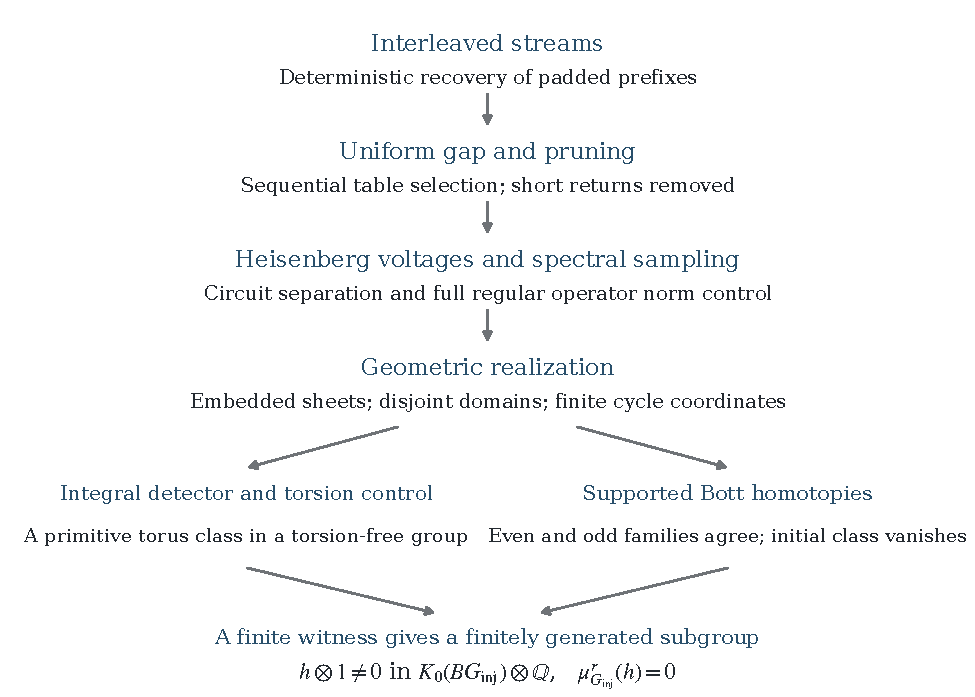
\includegraphics[width=\linewidth]{figures/proof-dependencies.pdf}
  \caption{Principal dependencies in the construction. The stream rules,
  sequential selection, and pruning precede the joint voltage and spectral
  choice. Geometric realization supports both the integral detector and
  the reduced Bott cancellation. A finite witness retains both properties
  in a finitely generated subgroup.}
  \label{fig:proof-dependencies}
\end{figure}

\subsection{Reading the construction}

There are two indices: height runs through one infinite graph tower,
while accuracy indexes a sequence of increasingly precise constructions.
The graph degree is constant across heights in any one construction and
may increase with accuracy. Section~\ref{sec:completion} records the
complete order of parameter choices after the required objects have been
defined.

Sections~\ref{sec:labeling}--\ref{sec:analysis} construct and sample the
labeled voltage tower. Sections~\ref{sec:geometry}--\ref{sec:domains}
realize it in a group and prove the cohomological detector and torsion
claims. Section~\ref{sec:assembly} establishes the reduced Bott
cancellation and extracts a finite witness. The final section puts these
conclusions together with compatible parameters and identifies the
detected torus Dirac class and its assembly image.

Throughout, all group $C^*$-algebras and all $K$-groups are complex.
Commutators mean $[a,b]=aba^{-1}b^{-1}$.  The graph construction uses
binary logarithms.  Matrix dimensions remain fixed along each
approximation sequence in which quotient $K$-theory is used; finite
generation is extracted only after an exact finite witness has been
obtained.
